\documentclass[11pt]{article}
\usepackage[utf8]{inputenc}
\usepackage[english]{babel}
\usepackage{bilal2vec}
\usepackage{minted}

\title{CS 480 - Notes}
\author{Bilal Khan (b54khan)\\
\href{mailto:bilal.khan@student.uwaterloo.ca}{bilal.khan@student.uwaterloo.ca}}
\date{\today}

\begin{document}

\maketitle

\paragraph{Perceptron Algorithm} If linearly separable with margin $\gamma$ and $||x|| \leq R$ convergence by update $k \leq R^2 / \gamma^2$. Can do one-vs-all (classifier for each class) or one-vs-one (classifier for each pair of classes)

\begin{minted}{python}
  y_hat = w.T @ x + b
  if y y_hat < delta:
    w = w + y x
    b = b + y
\end{minted}

\paragraph{Batch vs Online learning} Batch learning has IID data.

\paragraph{Empirical Risk Minimization} make probability large / make expected loss low $\argmin_w \frac{1}{n} \sum l_w(x_i, y_i)$

\paragraph{Regression} solve for grad 0. $A^T A$ not necessarily invertible

$$ \nabla_w L = 2 A^T A w - 2 A^T z $$
$$ \nabla^2_w L = 2 A^T a $$
$$ w = (A^T A)^{-1} A^T z $$

\paragraph{Jensen's Inequality} $f(\lambda x_1 + (1 - \lambda) x_2) \leq \lambda f(x_1) + (1 - \lambda) f(x_2)$. A twice-differentiable function is convex iff its Hessian is positive semidefinite everywhere. PSD matrices have non-negative determinants.

\paragraph{Convex} $M$ is convex if $v^T M v \geq 0$ for all $v$. grad zero $\leftrightarrow$ global minima if the function is convex. The least-squares loss is convex.

\paragraph{Ridge} $\lambda ||w||^2_2$

\paragraph{Lasso} $\lambda ||w||_1$

\paragraph{Gaussian} $p(x) = \frac{1}{\sqrt{2 \pi \sigma^2}} e^{- \frac{(x - \mu)^2}{2 \sigma^2}}$

\paragraph{Bernoulli} $p^k(1-p)^{1-k}$

\paragraph{Covariance} $E[X - E[X]]^T E[X - E[X]]$, symmetric + PSD

$$\dfrac{1}{\sqrt{2 \pi \text{det}[\Sigma]}} e^{-\frac{1}{2} (X - \mu)^T \Sigma^{-1} (X - \mu)} $$

\paragraph{Bayes} $p(x, y) = p(y | x)p(x)$

\paragraph{Likelihood} $\mathcal{L}(\mu, \sigma | x) = \Pi \dfrac{1}{2 \pi \sigma^2} e^{-\frac{(x_i - \mu)^2}{2 \sigma^2}}$

\paragraph{MLE} when predicting $\mu = Wx$, log likelihood, grad, set to zero, solve for $mu, \sigma^2$. For a Gaussian:

$$\hat{\mu} = \dfrac{1}{n} \sigma x_i$$
$$\hat{\sigma^2} = \dfrac{1}{n} \sigma (x_i - \mu)^2$$

For Bernoulli: $\hat{p} = (1/n) y_i$

\paragraph{MAP} Maximize the posterior using information about the prior. posterior = likelihood x prior

\paragraph{Entropy} uncertainty in a distribution. expectation of negative log P(x). Gaussian: $1/2 \log (2 \pi e \sigma^2)$. Bernoulli: $p \log p + (1 - p) \log(1 - p)$

\paragraph{KLD} difference between distributions/relative entropy $D_{KL} (P || Q) = P(x) \log (P(x) / Q(x))$

\paragraph{Kernel Density Estimation} $p(x) = \dfrac{1}{n \lambda} \sum K_\lambda (x, x_i)$

\paragraph{KNN classification} Classify new point with majority vote of K nearest neighbor's classes.

\paragraph{bias variance tradeoff} High bias (underfitting to complex model) vs high variance (overfitting to data points)

\paragraph{Curse of dimensionality} max distance decreases exponentially in higher dimensions

\paragraph{valid kernel} symmetric, distance fn $f(x, z) = f(x, y) + f(y, z)$, similarity measure $f(x, x) = 1$.

\paragraph{KNN clustering}

$$\min_{C_1, \cdots, C_k} \sum_{j=1}^{k} \dfrac{1}{|C_j|} \sum_{x_i, x_i^\prime \in C_j} ||x_i - x_i^\prime||_2^2$$
$$\mu_j = \dfrac{1}{|C_j|} \sum_{x_i \in C_j} x_i \text{Centroid}$$
$$\min_{C_1, \cdots, C_k} \sum_{j=1}^{k} \dfrac{1}{|C_j|} \sum_{x_i \in C_j} ||x_i - \mu_j||_2^2$$

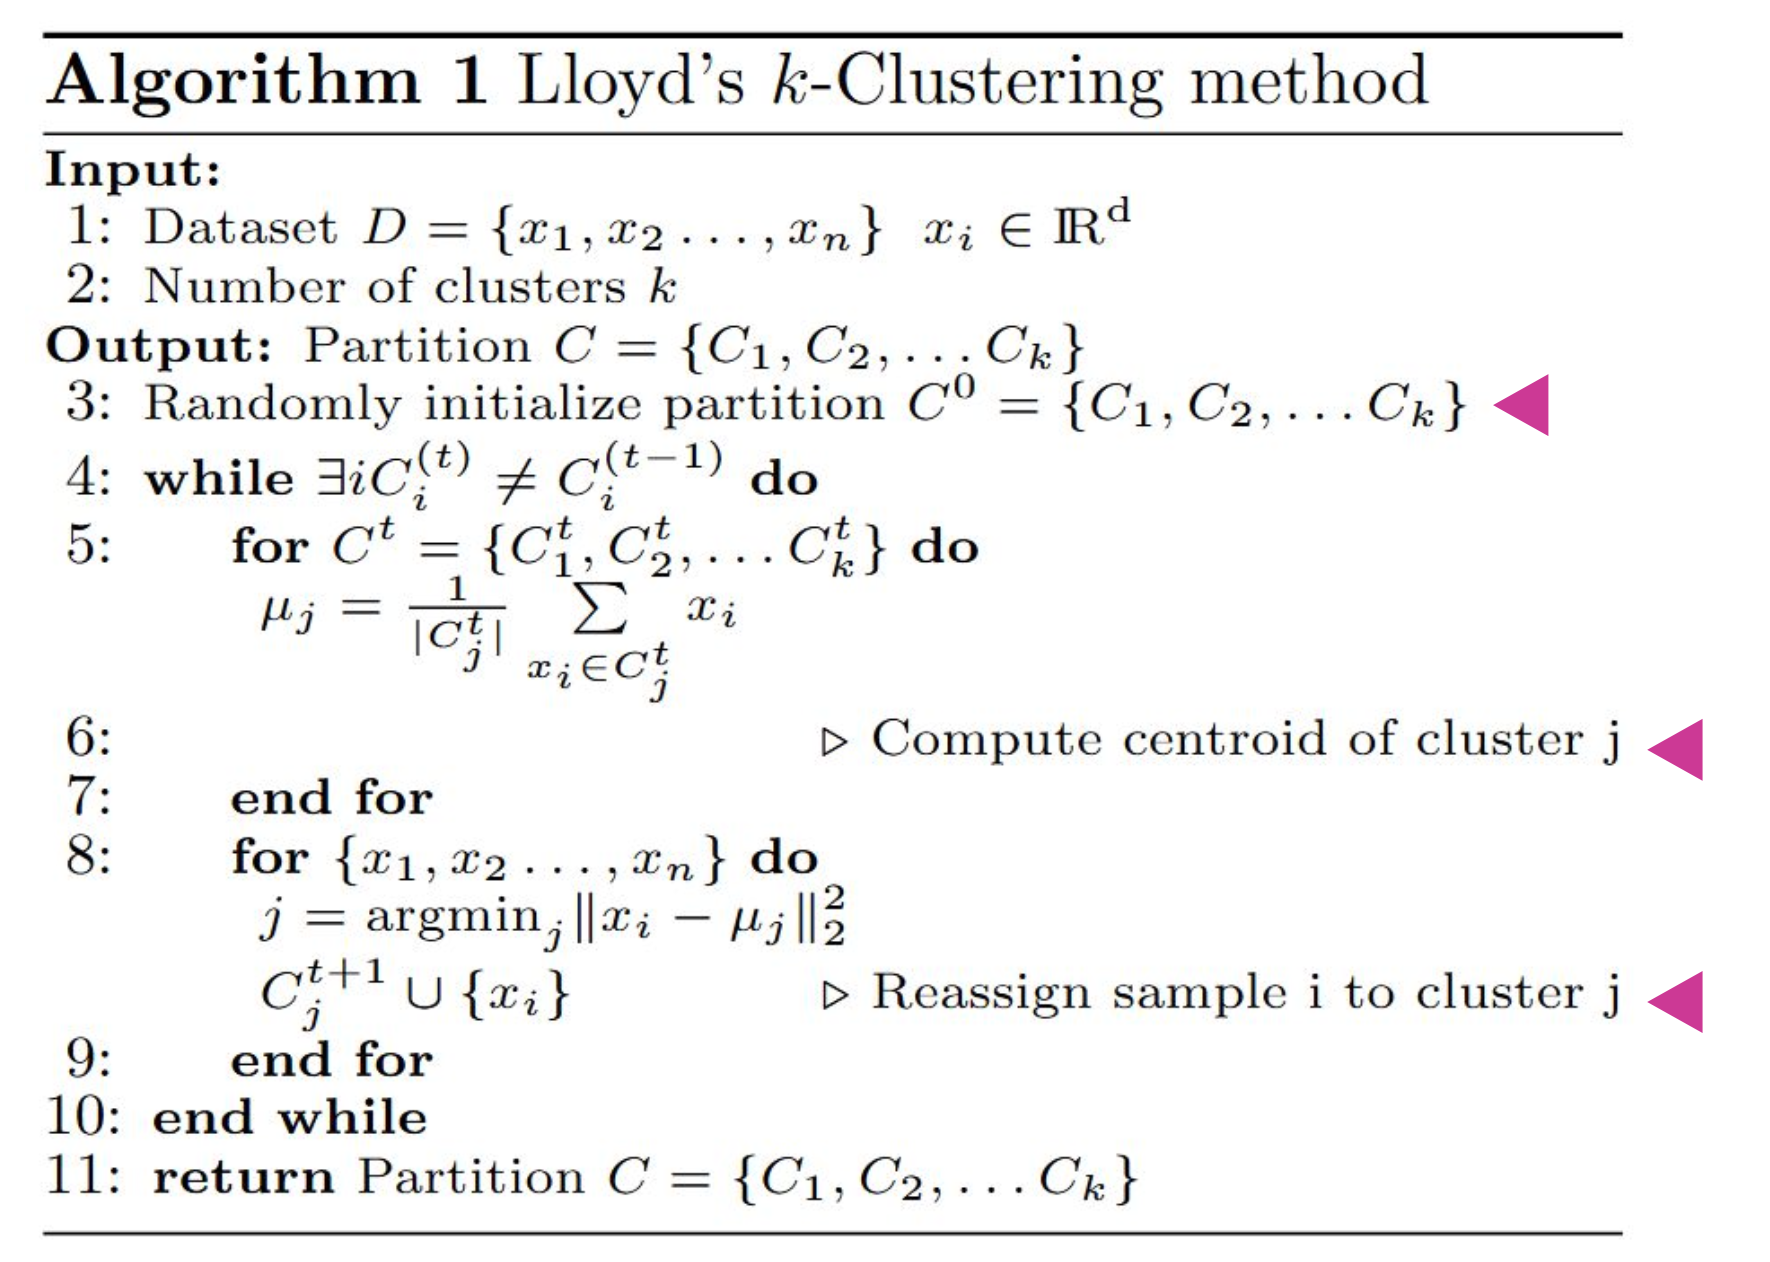
\includegraphics[width=400pt]{one.png}

\paragraph{Logistic Regression}

$$p(x) = \dfrac{1}{1 - e^{-w \cdot x}}$$

\paragraph{Logistic Regression LLH}

$$\log \mathcal{L} (w | x, y) = \sum_{i=0}^n - \log \left(1 + e^{\hat{y} (w \cdot x_i)}\right) $$

\paragraph{Newton's method} $w_1 = w_0 - \dfrac{f^\prime(w_0)}{f^{\prime\prime}(w_0)}$

\paragraph{Softmax} $\dfrac{e^{w_k \cdot x_i}}{\sum_{i=0}^c e^{w_i \cdot x}}$

\paragraph{Distance} between point and decision boundary: $d = \dfrac{w^T x + b}{||w||}$

\paragraph{Margin} is min distance over all points

\paragraph{Maximum margin problem} $\hat{w}, \hat{b} = \argmax_{w, b} \dfrac{1}{||w||} \min_{i} y_i (w^T x_i + b)$

\paragraph{As a constrained optimization problem} $\hat{w}, \hat{b} = \argmin_{w, b} \frac{1}{2} ||w||^2$ st $y_i (w^T x_i + b) \geq 1 \forall i$

\paragraph{Lagrangian dual} 

$$\min_{w, b} \max_{\lambda \geq 0} \mathcal{L}(w, b, \lambda) = \frac{1}{2} ||w||^2 - \sum_{i=1}^n \lambda_i (y_i (w^T x_i + b) - 1)$$

\paragraph{Soft-margin SVM}

This is the hinge loss

$$\hat{w}, \hat{b} = \argmin_{w, b} \frac{1}{2} ||w||^2 + C \sum_{i=1}^n \max(0, 1 - y_i (w^T x_i + b))$$

$$w = \sum_{i=1}^N \lambda_i y_i x_i$$ 

It has the same objective loss fn as hard-margin, but $0 \leq \lambda \leq C$ while hard-margin is $\lambda \geq 0$

\paragraph{Classification} Incorrectly, weakly correct (in decision boundary), strongly correct

\paragraph{Mercer kernels} Able to be written as a dot product of a function of each input. equivalent to the kernel function being positive semidefinite

\paragraph{Determinant} $1/(ad-bc) [d, -b, -c, a]$

\paragraph{SVM} 

$$\min_{0 \leq \lambda_i \leq C} \frac{1}{2} \sum_{i=1}^n \sum_{j=1}^n \lambda_i \lambda_j y_i y_j k(x_i, x_j) - \sum_{i=1}^n \lambda_i$$ st $\sum_{i=0}^n \lambda_i y_i = 0$.

\paragraph{Beta distribution}

$$\dfrac{\pi^{\alpha - 1} (1 - \pi)^{\beta - 1}}{\sum \pi^{\alpha - 1} (1 - \pi)^{\beta - 1}}$$

$$p(\pi) = \pi^{\alpha - 1} (1 - \pi)^{\beta - 1}$$

$$E[\pi] = \alpha / (\alpha + \beta)$$

Beta w a bernoulli prior:

$$p(\pi | y) = Beta(k + \alpha, n - k + \beta)$$

MAP estimate is then the expectation of $p(\pi | y)$

\paragraph{Bayesian Linear regression}

$$\bar{w} = A^{-1} (1 / \sigma^2) X^T y$$
$$A = \sigma^{-2} X^T X + \Sigma^{-1}$$
$$p(w | X, y) = N(\bar{w}, A^{-1})$$

Prediction:

$$p(y^\star | x^\star, X, y) = N((x^\star)^T \bar{w}, \sigma^2 + (x^\star)^T A^{-1} x^star)$$

\paragraph{Gaussian processes} 

$$t_i = y_i + \epsilon_i$$
$$C_{ij} = \alpha^{-1} k(x_i, x_j) + \beta^{-1} \delta_{ij}$$
$$p(t) = N(t | 0, C)$$
$$p(y) = N(y | 0, \alpha^{-1} K)$$
$$p(t | y) = N(t | y, \beta^{-1} I_n)$$

\paragraph{prediction} 

$$p(t_{N+1}) = N(t_{N+1} | 0, C_{N+1})$$
$$C_{N+1} = [C_n, k, k^T, c]$$
$$k = [\alpha^{-1} k(x_1, x_{N+1}), \cdots]$$
$$c = \alpha^{-1} k(x_{N+1}, x_{N+1}) + \beta^{-1}$$
$$\mu_{N+1} = k^T C_N^{-1} t$$
$$\sigma^2_{N+1} = c - k^T C^{-1} k$$

\paragraph{Decision Tree}

Predict by majority vote of class in new point's region

\paragraph{Gini index} $\sum p_{mk} (1 - p_{mk})$

\paragraph{Bootstrapping} Reduce variance by resampling original data with replacement

\paragraph{Bootstrap Aggregation (Bagging)} Aggregate of multiple predictions, Can resample observations or features. Reduces variance when prediction errors are uncorrelated.

\paragraph{Boosting} Sequentially trained ensembles can be used to reduce bias as well. 

\paragraph{Expectation Maximization}

Estimate data parameters with latent variables. Compute expecation of latent variables given current parameters. Use them to compute parameters that maximize the log likelihood of the data.

In practice.

$$\mathcal{L}(\theta_t) = \sum \log p(y | \theta_t)$$
$$\theta_{t+1} = \argmax_{\theta} \sum \log p(y | \theta_t)$$
$$\ell_t(\theta) \geq \sum_n \left[ - D_{KL} (q_n(z_n) || p(z_n | y_n, \theta)) + \log p(y_n | \theta) \right]$$


$$\hat{\gamma}_i = \dfrac{\pi \mathcal{N}_{\mu_2, \sigma_2^2} (x_i)}{(1 - \pi) \mathcal{N}_{\mu_1, \sigma_1^2} (x_i) + \pi \mathcal{N}_{\mu_2, \sigma_2^2} (x_i)}$$

$$\hat{\pi} = \frac{\sum_{i=1}^N \hat{\gamma_i}}{N}$$
$$\hat{\mu}_1 = \frac{\sum_{i=1}^N (1 - \hat{\gamma}_i) y_i}{\sum_{i=1}^N (1 - \hat{\gamma}_i)}$$
$$\hat{\mu}_2 = \frac{\sum_{i=1}^N \hat{\gamma}_i y_i}{\sum_{i=1}^N \hat{\gamma}_i}$$
$$\hat{\sigma^2}_1 = \frac{\sum_{i=1}^N (1 - \hat{\gamma}_i) (y_i - \hat{\mu}_1)^2}{\sum_{i=1}^N (1 - \hat{\gamma}_i)} $$
$$\hat{\sigma^2}_2 = \frac{\sum_{i=1}^N \hat{\gamma}_i (y_i - \hat{\mu}_2)^2}{\sum_{i=1}^N \hat{\gamma}_i} $$

\paragraph{Jensen's Inequality} $\log E_{q_n} [Z] \geq E_{q_n} [\log Z]$ 

\paragraph{Regularization} Early stopping, weight decay, augmentation, dropout

\paragraph{Normalization} Consistent scale, large enough batch size, IID required

\paragraph{CNN} Locality, spatial invariance. $W_{out} = W_{in} + 2 P - F) / S + 1$. Translation equivariant (adaps) (pooling) but not invariant (ignores)


\end{document}
